%\chapter{Optimizing SNSPD HBT and TCSPC measurement of a fs pulsed source}
\chapter{Optimization of SNSPD-Based HBT and TCSPC measurements with a femtosecond pulsed source}
\label{Capitolo4}

In this chapter will be presented the procedures carried out to optimize the HBT and TCSPC measurements that we took with a femtosecond pulsed laser source.
In detail, \autoref{cpp:Motivations} provides the reader the driving motivations as well as a description of the experimental setup we used.
Moving forward with the structure of the chapter, \autoref{cpp:Initial-khaos} provides conditions, observations and conclusions behind the first chaotic measurement obtained with this setting.
Lastly, \autoref{cpp:Improvements&discussion} brings to the discussion the driving idea behind the troubleshooting, together with a qualitative discussion of the results obtained after such changes.



\section{Motivations and experimental setup overview}
\label{cpp:Motivations}
When studying pulsed laser light with the use of an SNSPD as a detector, it is good practice to question the results obtained with respect to the various jitter sources involved. Isolating such timing jitter sources can be a difficult task. For this reason a good approach can involve changing the pulsed laser light to another whose jitter is known, or also negligible under certain circumstances. By choosing this approach we substantially simplify the recognition of all the other jitter sources involved outside of the pulse generation jitter, providing an optimal setup to quantify the precision of the detection instrument. 
In this second part of this thesis we will then present the procedures of optimization that we carried out on HBT and TCSPC measurements obtained with a femtosecond pulsed laser, whose intrinsic jitter can easily be considered negligible when compared to the laser source of the first part.

In particular, the laser source we used is a mode-locked Titanium-Sapphire (Ti:Sa) laser, driven by a 6.34~W Sprout-G-15W laser manufactured by Lighthouse Photonics. Under these working conditions the Ti:Sa is capable of producing $\leq 100$~fs pulses. An important remark needs to be made about this temporal duration : although the manufacturer specifies that with a 5~W pump laser the output pulses can reach $\sim 50$~fs, these values correspond to nearly transform-limited pulses under optimal cavity alignment and dispersion compensation. In our case the output was not transform-limited, so we treated the Ti:Sa as a black box. The only verification we carried out on this black box relied on the real time spectrum of the laser. From the spectral measurement we were able to identify the operating wavelength, the spectral width and above all confirm the pulsed regime. In the case of a spectrum without a distinct peak, we would have concluded that the Ti:Sa was producing CW output instead of the desired pulsed regime.

The key differences with respect to the experimental setup presented in \autoref{sec:Overview} can be summarized as follows:
\begin{itemize}
    \item Ti:Sa femtosecond pulses replacing the previous EOM-driven source,
    \item Single-mode fiber (Thorlabs 780HP) instead of the polarization-maintaining fiber,
    \item TCSPC operated with a divided SYNC provided by a multifunctional divider box, yielding an effective frequency at the ID1000 of about 20~MHz.
\end{itemize}

An overview of the experimental setup is shown in \autoref{TisaSetup}. The sketch does not include the attenuation stage placed before the fiber coupler, which is a fundamental part of the setup. This stage was specifically required to reduce the power from the original 0.1~W at the Ti:Sa output to roughly one quarter of that value. This downsizing was possible thanks to the use of a prism and a beam splitter, together with two infringing barriers. All these elements were properly positioned to direct only the last quarter of power into the fiber coupler.

%An overview of the experimental setup can be found in \autoref{TisaSetup}, though the sketch misses the part of the setup designed to attenuate the power before the fiber coupler. Although not depicted in the image, this is a fundamental part of the setup, specifically required to lower the power from the original 0.1~W at the raw exit of the Ti:Sa to roughly a quarter of it.

\begin{figure}[hbtp]
\centering
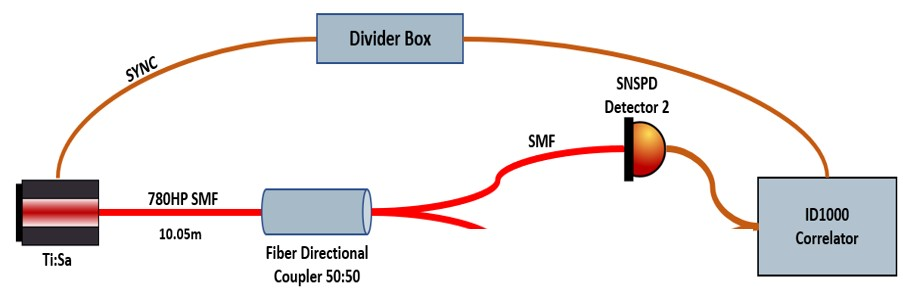
\includegraphics[width=1\textwidth]{TiSa_Setup.jpg}
\caption{Visual representation of the experimental setup. The pulsed output of the Ti:Sa laser (left) propagates through $\approx 10$~m of single-mode fiber (SMF) before reaching a fiber directional coupler. The beam is then divided into two channels that are directed to separate inputs of the SNSPD. Detection events are collected by the ID1000 time-tagger. Also shown are the electronic cables linking the Ti:Sa electronic pulser to the ID1000 via a multifunctional divider box.}
\label{TisaSetup}
\end{figure}




\section{Undesired Side Peaks in HBT and TCSPC measurements}
\label{cpp:Initial-khaos}
Up to this point in the discussion, we can now start presenting the data from the measurements.  
The first measurement was taken with an exposure time of 10~s, under conditions of approximately 3~MCounts detected. Regardless of the divided SYNC signal sent to the ID1000 at $\sim 20$~MHz, the actual repetition rate of the pulsed laser was 80~MHz.  

Assuming output pulses of $\approx 100$~fs, as discussed in the previous section, the fiber dispersion broadens them to $\approx 23$~ps at the SNSPD input. The resulting histograms are shown in \autoref{Khaos}, where each main peak is shifted to the center of the time axis, and the counts are displayed on a logarithmic y-axis.  

From these histograms, two key observations can be made:  
\begin{itemize}
	\item Although very similar overall, Detector~3 registers slightly more events than Detector~2, as indicated by the red main peak being $18.6\%$ higher than the black one;
	\item Side peaks appear at different relative times for the two detectors, but the $-500$~ps peak is consistently present across all four histograms.
\end{itemize}

From this first inspection, the conclusion is clear: before proceeding with further measurements, it is necessary to better characterize the origin of the side peaks observed here.


%with a non negligible number of side peaks appearing, it was necessary to take a step back to try assess the


\begin{comment}
At a regime of 3~MHz we ran the first set of measurements, over a time of 15s of exposure time.
The resulting histograms are then post-processed to shift the main peak in the zero time position, in order to ease the comparison between the different peaks.
\autoref{Khaos} shows the chaotic situation we got with the first measurement. So many side peaks appear, and the situation is far to be understood.

\end{comment}

\begin{figure}[hbtp]
\centering
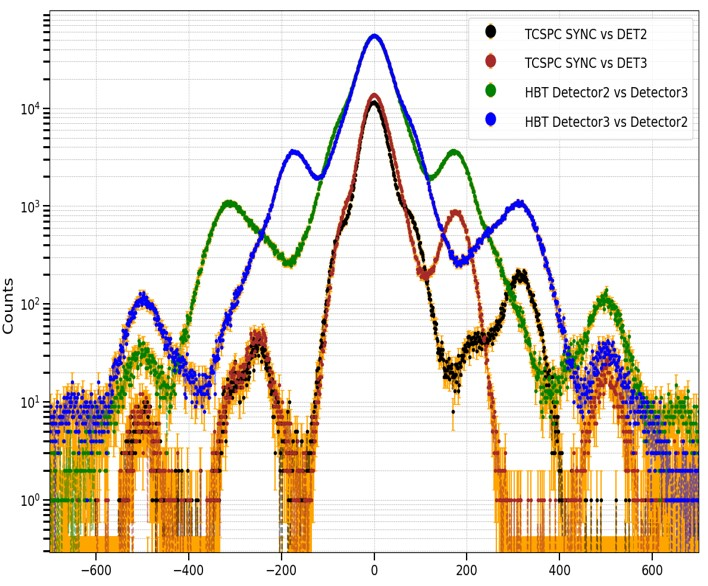
\includegraphics[width=1\textwidth]{Khaos.jpg}
\caption{Measured TCSPC and HBT Histograms, post processed to display the main peak in the origin of the time axis to ease confrontation. Counts are displayed in the y-axis using a logarithmic scale. The two TCSPC histograms related to Detector~2 and Detector~3 are represented in black and red respectively. The two HBT histograms are displayed in green and blue.}
\label{Khaos}
\end{figure}

\section{Partly retrieving side peaks in HBT from coordinates of TCSPC peaks}
\label{cpp:Reconstructsides}
Explaining side peaks of a set of TCSPC and HBT histograms can be challenging. 
This scenario needs to be approached carefully, starting from the basic information available in the histograms. As discussed in \autoref{sec:Def-Techniques}, the histograms from the two start/stop HBT measurements are directly related to the TCSPC plots of the individual detectors.
Focusing on \autoref{Khaos}, we notice that the total number of side peaks is higher in the HBT measurements. This occurs because the HBT setup amplifies the side peaks already present in the TCSPC data from the individual detectors, as seen in the red and black plots. 

What we observe in \autoref{Khaos} can be explained mathematically by Eqs.~ \ref{TCSPC_convo} and \ref{HBT_convo} as follows :
\begin{equation}
TCSPC_{Det.2}(t) = I(t) \circledast IRF_{Det.2}(t)
\label{TCSPC_convo}
\end{equation}

\begin{equation}
HBT_{2,3}(t) = I(t) \circledast IRF_{Det.2}(t) \circledast IRF_{Det.3}(t)
\label{HBT_convo}
\end{equation}

The twofold convolution in \autoref{HBT_convo} makes it possible to qualitatively identify the HBT side peaks from the coordinates of the summits observed in the two separate TCSPC histograms.
Although qualitative, this procedure requires the time coordinates of every peak with reasonable accuracy.
A natural starting point is therefore to label each peak; from now on we adopt the labeling convention introduced in \autoref{Khaos_labeled}.
The corresponding numerical values are summarized in \autoref{tabellonadeipicchi}.

With this framework in place, the next step is to compute sums and differences of the C- and D-class peak coordinates, collecting the valid combinations in a list.
Among the several side peaks observed, four HBT peaks can be successfully identified through this procedure:
\begin{itemize}
\item $D0 - C1$ corresponds to the position of $A2$
\item $C1 - D0$ corresponds to the position of $B2$
\item $D1 - C0$ corresponds to the position of $A1$
\item $C0 - D1$ corresponds to the position of $B1$
\item The absence of $C4$ accounts for the reduced height of $A3$ relative to $B4$
\end{itemize}
These four identifications also serve as a direct confirmation that, by inverting the operations, one retrieves the positions of the corresponding peaks in the time-reversed HBT histogram. The hierarchical convention chosen for the numbering of the labels reinforces this interpretation: in both of the first two operations the resulting index is the same (2), and the same scheme applies to the third and fourth operations.



%Due to the convolution operator, these equations allow us to relate the peaks of the HBT histograms to the relative time coordinates of the TCSPC peaks.
%The main reason behind the possibility of reaching an explanation of the HBT peaks, from the TCSPC ones lies in the convolution operator, appearing twice, that relates the two detectors in 
\begin{figure}[hbtp]
\centering
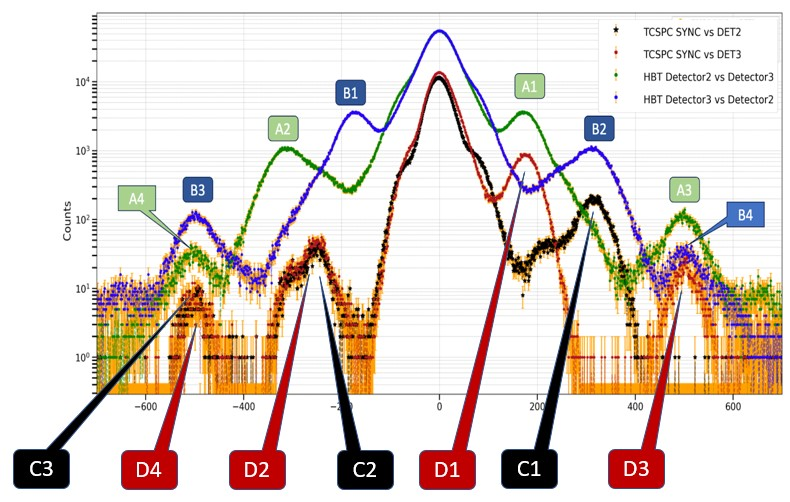
\includegraphics[width=1\textwidth]{Khaos_Labeled.jpg}
\caption{Labeled version of \autoref{Khaos}. Each peak is labeled using the same color as its corresponding histogram. Numbers are assigned to indicate hierarchical relations between side peaks of the same color. The central peak is not labeled, but within this scheme it would correspond to the index zero.}
\label{Khaos_labeled}
\end{figure}


\begin{table}[h!]
\centering
\caption{\textbf{Detected position of the peaks}}
\renewcommand{\arraystretch}{1.3}
\begin{tabular}{
>{\centering\arraybackslash}m{1.5cm} 
>{\centering\arraybackslash}m{1.5cm} 
>{\centering\arraybackslash}m{1.5cm} 
>{\centering\arraybackslash}m{1.5cm} 
>{\centering\arraybackslash}m{1.5cm}}
\rowcolor{blue!50}
\textcolor{white}{\small[\textbf{ps}]} & \textcolor{white}{\textbf{A}} & \textcolor{white}{\textbf{B}} & \textcolor{white}{\textbf{C}} & \textcolor{white}{\textbf{D}} \\
\rowcolor{white}
\cellcolor{blue!50} \textcolor{white}{\textbf{0}} & 0    & 0    & 0     & 0     \\
\rowcolor{white}
\cellcolor{blue!50} \textcolor{white}{\textbf{1}} & 174  & -174 & 316   & 175   \\
\rowcolor{white}
\cellcolor{blue!50} \textcolor{white}{\textbf{2}} & -313 & 312  & -250  & -246  \\
\rowcolor{white}
\cellcolor{blue!50} \textcolor{white}{\textbf{3}} & 495  & -494 & -500  & +501  \\
\rowcolor{white}
\cellcolor{blue!50} \textcolor{white}{\textbf{4}} & -502 & 503  & n.d.  & -500  \\
\rowcolor{white}
\end{tabular}
\label{tabellonadeipicchi}
\end{table}









\section{Measurements with improved detection thresholds}
\label{cpp:Improvements&discussion}
This section is dedicated to the refinement of a cleaner dataset, with the ultimate goal represented by dataset possibly free of undesired side peaks.
Achieving such result would allow further analyses to be made, starting from the deconvolution of the IRF, for example.
Among the different approaches we tried, we will be presenting here only the most effective one, with a final discussion at the end.


\subsection{Driving idea}
Among other possible components of the setup and considering the relative distance between the central peak and the side ones, we focused primarily onto the electronic framework that plays a role after the SNSPD.
This focus on the electronic cables and equipment is motivated by the specifications of the SNSPD: the detector’s deadtime is on the order of nanoseconds, far larger than the picosecond separation between the peaks, making it impossible for the side peaks to arise from double detection events.
A more plausible explanation is an inappropriate choice of electronic thresholds in the ID1000, causing multiple clicks to be registered from a single SNSPD detection event.
Analyzing the electronic pulses generated by the SNSPD is then a clear first step to assess the correctness of such thresholds.
Up until this point, all measurements we took had the ID1000 set on triggering each time the falling edge of the pulse dips below -100mV.

To analyze the electronic signal, we plugged one at a time the output cables of our two SNSPD channels into the oscilloscope. An impedance reduction of 50~$\Omega$ was added before the scope port, to match the behavior that reaches the time tagger.
In this context, \autoref{TrickShot} shows oscilloscope screenshots of the electronic signals from Detectors 2 and 3, displayed on the left and right panels, respectively.
Important to mention, each one of these observations was conducted in conditions of very low counts, resulting from some stray photons in the laboratory.
In these two images two lines can be appreciated: a yellow line corresponding to the average between 100 pulses of the electronic signal shape, as well as a light-blue line representing the oscilloscope-derived first derivative.

The new thresholds were set to reflect the point of maximum steepness of the falling edge, as indicated by the first derivative (light blue trace).
In \autoref{TrickShot}, the previous and newly chosen thresholds are indicated in red and green, corresponding to \(-500\)~mV and \(-600\)~mV, respectively.
This adjustment strengthens the signal-to-noise ratio, suppressing undesired clicks that might otherwise arise from small oscillations or late resonances in the electronic pulse following the main peak, as also illustrated in \autoref{TrickShot}.




\begin{comment}
%Above other possible explanations and considering the small time intervals between the central peak and the other side summits, we concluded that the first part of the setup to analyze had to be the electronic one.
%We base this suspicion on behalf of the deadtime of the detector : the manufacturer states that the recovery time before the nanowire is ready to detect an event after the previous one is far greater than the relative intervals we see in \autoref{Khaos}. It is then highly difficult that the physical reason behind those side peaks is some sort of afterpulsing. 
%These hypotheses led us to the analysis of the electronic pulses generated by the SNSPD, to understand whether the settings were correct or not.
%of the second detector into an oscilloscope, making sure to add an impedance of 50~$\Omega$ to match the signal that was effectively reaching the time tagger.



we strongly suspect that the chaotic behavior that we're getting, although we're visualizing the data always in log scale finds its origin in a sort of miscalibration of the triggering thresholds.
For this reason we managed to shut the laser and while the detector was receiving only stray photons, we looked at the electronic pulses coming out of the SNSPD.
Subsequently we initialized the Oscilloscope to visualize also the first derivative of the pulse so that we could get an info on where to locate the new, and refined threshold. The whole idea was to choose the point where the electrical signal expressed the greatest steepness, in order to achieve better measurements.
The whole idea we formulated explained the side peaks, as a consequence of having the detector measuring clicks when it was not fully recovered from the previous detection. By Modifying for a stronger threshold, as seen in \autoref{TrickShot}, we are getting rid of the even slow possibility to trigger with a non fully recovered nanowire.
Important mention is related to how we looked at these signals : instead of plugging the cable from the SNSPD straight into the Oscilloscope, we managed to add an impedance load to it, valued $50 \Omega$, to simulate the impedence that it will encounter at the entrance of the ID1000 Time-Tagger.
\end{comment}


\begin{figure}[hbtp]
\centering
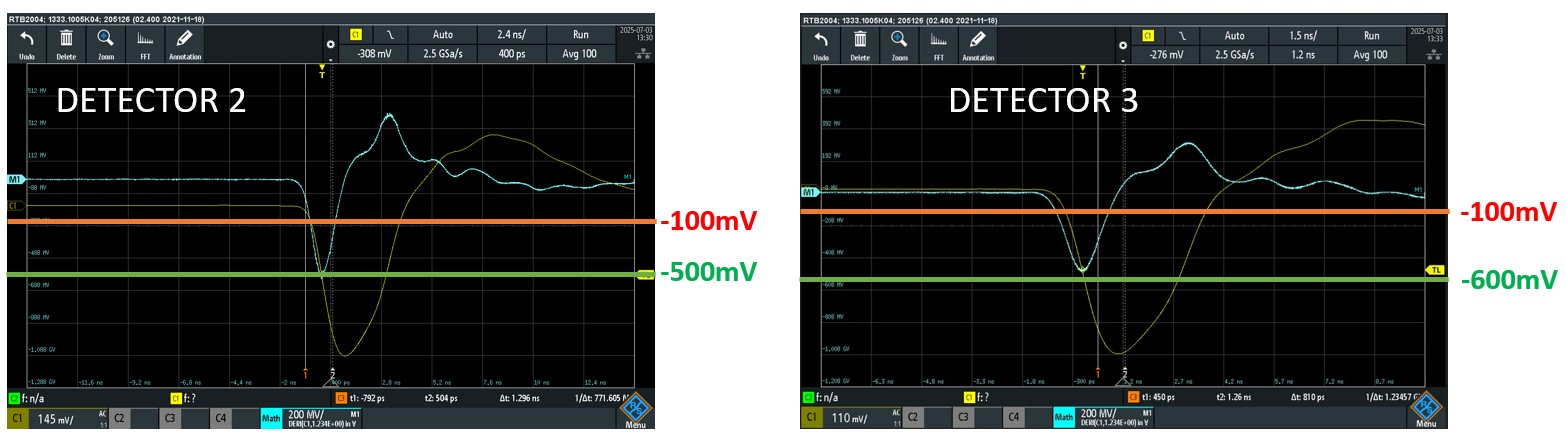
\includegraphics[width=1\textwidth]{ScopeShots.jpg}
\caption{Oscilloscope view of an electronic pulse generated from two different SNSPD detectors. Left image is related to the second detector, while the right one is instead related to the third. The yellow line represent the signal itself, while the blue line represents its first derivative. Both the images do show the past and the refined thresholds, respectively like orange and green lines.}
\label{TrickShot}
\end{figure}

\begin{comment}
As seen in \autoref{TrickShot}, by looking at the images we significantly modified the thresholds, passing from a value of $-100mV$ for both the detectors to $-500mV$ and $-600mV$, for detector 2 and detector 3 respectively.
\end{comment}


%\subsection{Discussion of the new measurements}
%After refining the new thresholds, a new and final set of measurements was taken.
%In this final section we will assess whether the choice of refining the electronic thresholds of the ID1000 is the decisive change needed to remove the undesired side peaks appearing in \autoref{Khaos}, or if otherwise there are no significant improvements.
%
%The final measurement was taken with a long exposure time of 500~s.
%Minimizing the impact of the noise in count-based histograms is a strategy that finds its roots in the intrinsic nature of the noise in the TCSPC and HBT histograms.
%As we introduced also in \autoref{subs:TCSPC}, the prevalent noise of these histograms scales with the square root of the number of counts, as also referenced in \autoref{SNR_TCSPC}.
%The signal itself scales instead like the number of counts itself. For this reason, longer exposure times mitigate the disruption caused by the shot noise, unveiling parts that because of low counts were highly affected by noise.
%Furthermore, external light coupled in the optical fibers was minimized turning off the lights, and the final count rates corresponded to $\approx 240$~kHz  for both the two detectors.
%The final histogram obtained is shown in \autoref{RefinedMeasurement}, where the usual color scheme is maintained (black and red for the two TCSPC; blue and green for the two HBT).
%Focusing on the image some key observations can be made :
%\begin{itemize}
%\item The strong similarity between the height of the two main peaks reflects the similar count rates mentioned above;
%\item The characterization of the main peak is substantially improved, much less side peaks are now present.
%\item The Red TCSPC, corresponding to the third detector still exhibits a persistent side peak, separated from the main one at approximately +500~ps
%\item Both of the main peaks of the two TCSPC histograms do not have similar tails. This particularly applies to the black one, where the distortion on the right tail is particularly evident.
%\item The second peak at +500~ps does not appear for the black histogram. 
%\end{itemize}
%
%
%
%In conclusion, was refining the electronic threshold an effective solution to remove the side peaks ?
%On behalf of the above observations, it is not possible to assess that the cause of the multiple side peaks appearing in \autoref{Khaos} was solely the use of wrong electronic thresholds.
%Though the characterization of the main peak has significantly improved, there is still room for improvement for both of the detectors.
%In particular for the third detector, it is to be further assessed the underlying reason for the presence of the separate peak at +500~ps after the main peak.


\subsection{Discussion of the new measurements}
After refining the electronic thresholds, a new and final set of measurements was taken.
In this section we assess whether this adjustment was the decisive change needed to remove the undesired side peaks observed in \autoref{Khaos}, or whether significant issues remain.

The final measurement was taken with a long exposure time of 500~s.
Since shot noise scales as the square root of the number of counts, while the signal itself scales linearly, longer exposure times improve the signal-to-noise ratio and reveal weaker structures otherwise buried in noise, as discussed in \autoref{subs:TCSPC} and \autoref{SNR_TCSPC}.
Furthermore, external light coupled into the optical fibers was minimized by switching off all laboratory lights, and the final count rates corresponded to $\approx 240$~kHz for both detectors.
The resulting histogram is shown in \autoref{RefinedMeasurement}, where the usual color scheme is maintained (black and red for the two TCSPC; blue and green for the two HBT).

From \autoref{RefinedMeasurement}, several key observations emerge:
\begin{itemize}
\item The strong similarity between the heights of the two main peaks reflects the nearly identical count rates.
\item The characterization of the main peak is substantially improved, and most side peaks are now suppressed.
\item Detector~3 (red TCSPC) still exhibits a persistent side peak at about +500~ps.
\item The main peaks of the two TCSPC histograms exhibit dissimilar tails; in particular, the right tail of the black trace shows a clear distortion.
\item The side peak at +500~ps does not appear in the black histogram.
\end{itemize}

In conclusion, refining the electronic threshold proved partially effective in reducing the undesired side peaks, but it was not sufficient to fully resolve the issue. 
Although the main peak characterization has improved significantly, the persistence of a secondary peak in the red TCSPC histogram and the distortions in the black trace indicate that further changes to the setup are necessary. 
The next step will therefore focus on additional modifications aimed at eliminating these residual artifacts and achieving clean TCSPC and HBT histograms.





%\begin{figure}[hbtp]
%\centering
%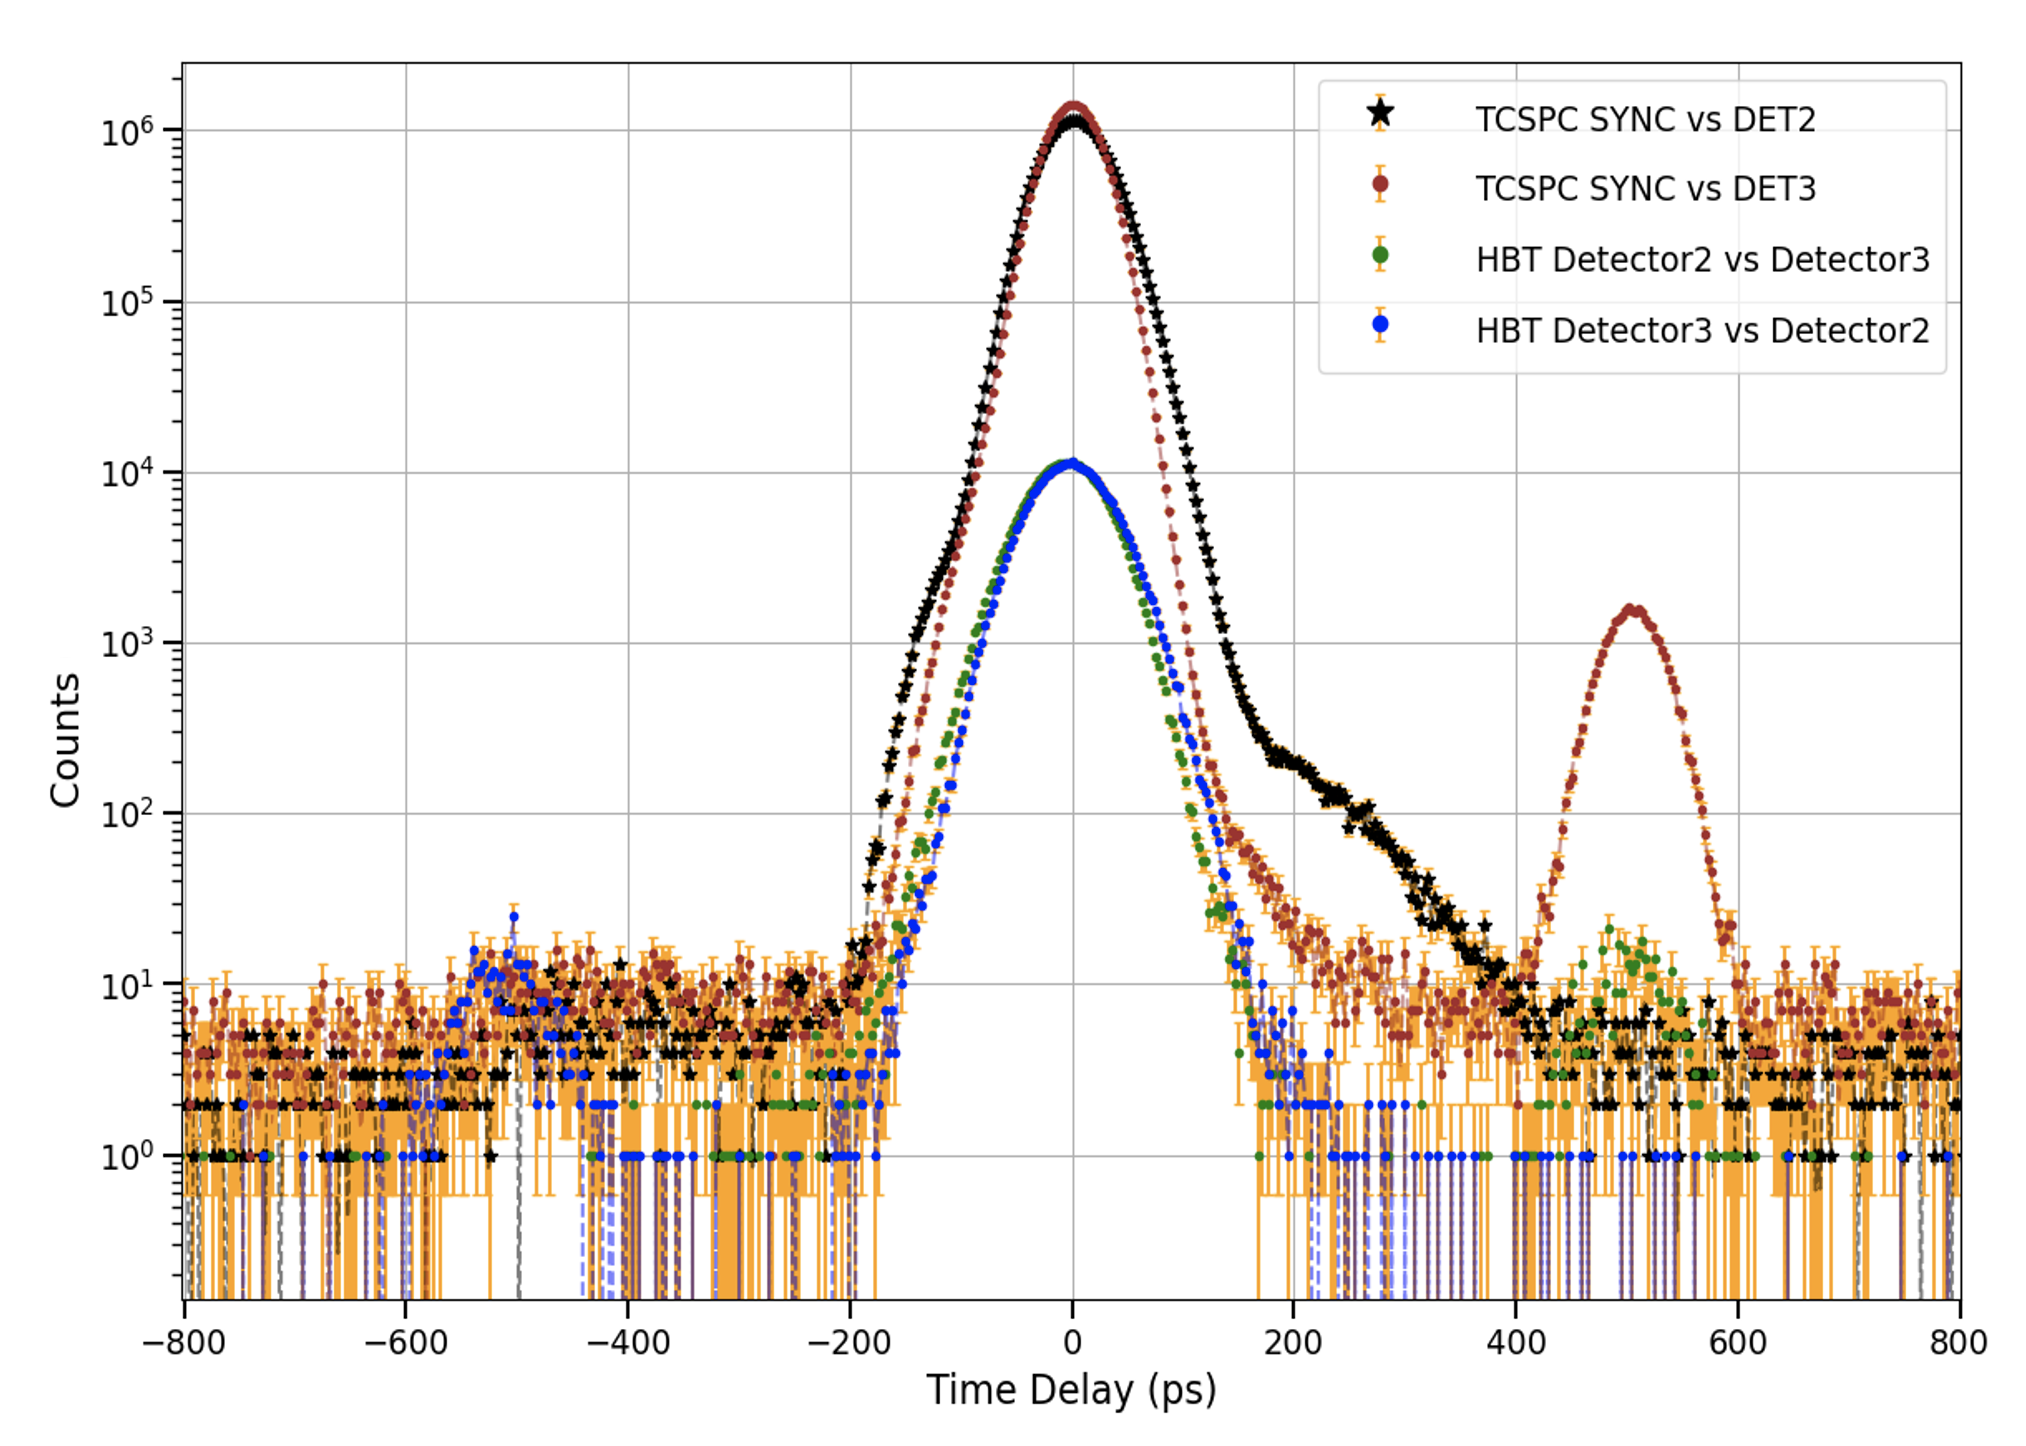
\includegraphics[width=1\textwidth]{Refined.jpg}
%\caption{Measured TCSPC and HBT Histograms corresponding to the measurement with the updated threshold values, specifically chosen to enhance the signal to noise ratio and remove undesired side peaks. Every peak has been shifted to appear in the center of the axis, and the counts are displayed in a logarithmic vertical scale. }
%\label{RefinedMeasurement}
%\end{figure}


%This final step is crucial to assess whether better thresholds actually improve the clarity of the main peak, maybe also solving completely the issue of the undesired side peaks, or instead does not make any difference.


\begin{comment}
Cose da dire qui in questa parte di tesi : 
1 ) Descrivere le condizioni in cui abbiamo eseguito queste ultime e finali misure
2 ) Fare le osservazioni che abbiamo scritto nel documento condiviso con anche W.
3 ) Trarre le conclusioni per quanto riguarda questa parte di tesi.


Svolgimento di queste parti :
Parte 1 )  [Se teniamo l'idea di presentare solo l'immagine con il countrate maggiore]
 a ) Countrate ai detector
 b ) Breve riferimento alla sezione precedente per definire le threshold utilizzate per questa parte
 c ) Tempo di esposizione, con conseguente  commento sulla quantità di noise che si vede dall'immagine che dovrebbe essere non esagerata per via per l'appunto della lunghezza
 d ) Condizioni laboratoriali in cui abbiamo effettuato le misure
 
 Parte 2 ) 
 a ) The two TCSPC have significantly improved upon the refinement of the thresholds
 b ) Det. 3 still shows a persistent separated peak at +500ps. this automatically creates also a small bump at -500ps in the det3 vs det2 HBT. completely understandable, and also in the det2 vs det 3 at exactly 500ps
 c ) The Det. 2 TCSPC has the right tail highly deformed by what appears to be an underlying side peak whose center could be something around 200ps ?!?!?!?!?
 d ) Also Detector 3 has the right tail deformed, but this time significantly less than the black's deformation.
 
 Parte 3 ) 
 Refinining better thresholds has significantly improved the quality of our measurements, making now possible to study better the main peak.
 Though the situation has significantly improved, DET3 's TCSPC still shows a persistent +500ps bump, as well as the black depicting a strongly deformed right tail.
 
 New thresholds have significantly improved the situation, though it appears that this is not totally resolutive.
\end{comment}



\begin{figure}[hbtp]
\centering
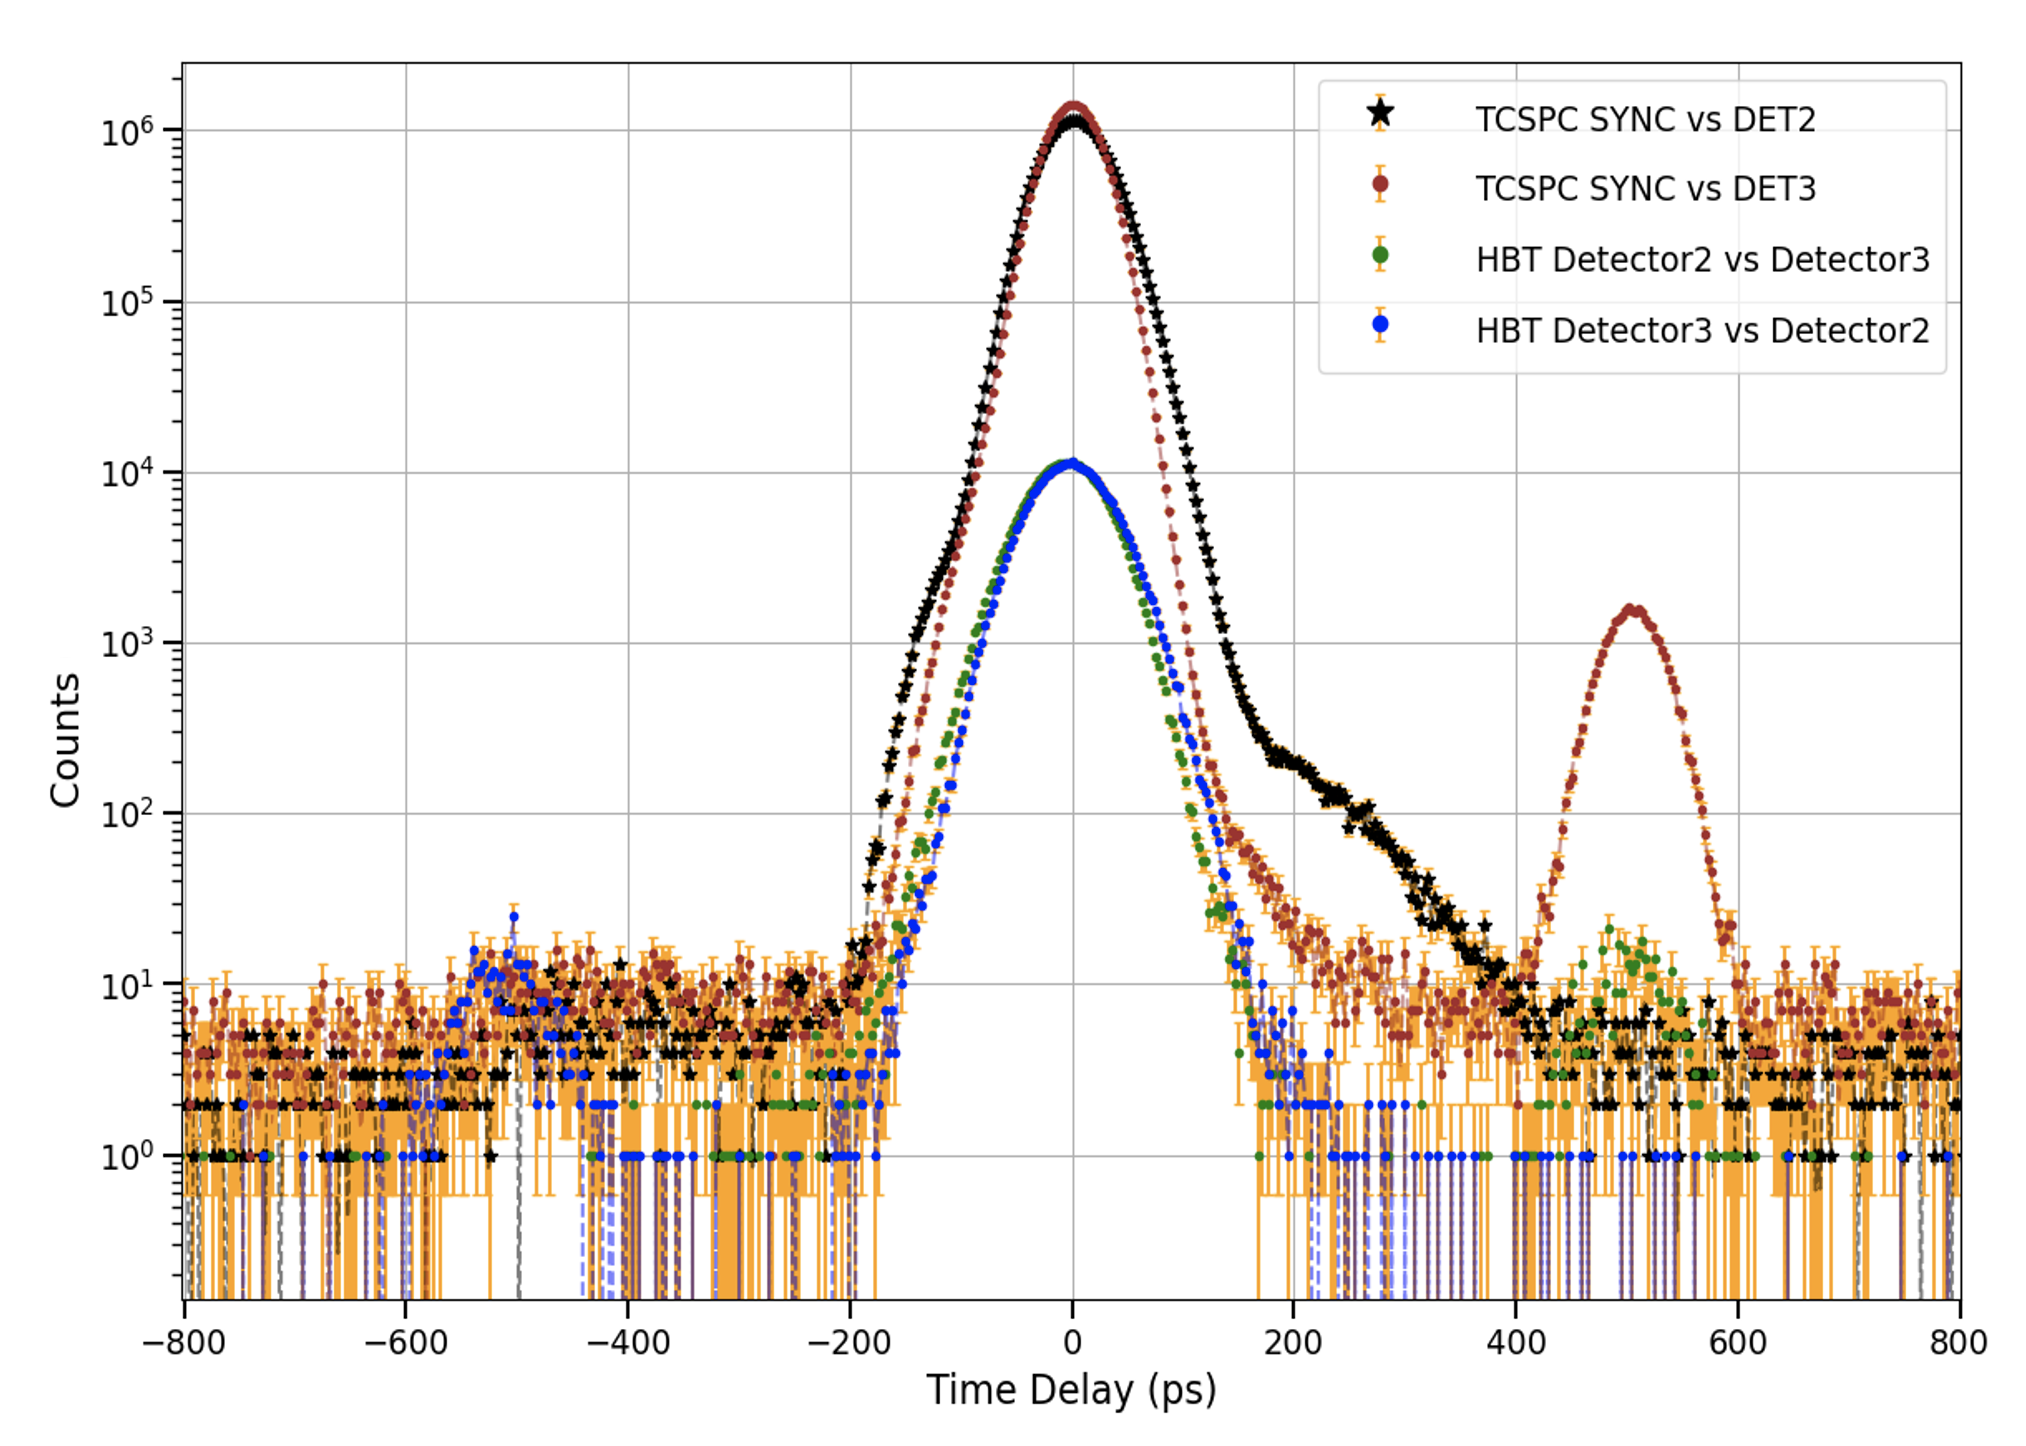
\includegraphics[width=1\textwidth]{Refined.jpg}
\caption{Measured TCSPC and HBT Histograms corresponding to the measurement with the updated threshold values, specifically chosen to enhance the signal to noise ratio and remove undesired side peaks. Every peak has been shifted to appear in the center of the axis, and the counts are displayed in a logarithmic vertical scale. }
\label{RefinedMeasurement}
\end{figure}


%  Although most of the side peaks are not appearing evidently like in \autoref{Khaos}, a clear side peaks still arises at +500ps  for the third detector TCSPC histogram.

% \subsection{Estimation of the width of the Detector response function}